\chapter{Πειράματα και Αποτελέσματα}
\label{ch:experiments_and_results}

\section{Υλικό διεξαγωγής πειραμάτων}
Για την εκτέλεση κώδικα με σκοπό την διεξαγωγή πειραμάτων απαιτείται η χρήση υπολογιστή ή μιας υπολογιστικής μονάδας. Στην υλοποίηση που απαιτείται για το αντικείμενο της συγκεκριμένης εργασίας ορισμένες διαδικασίες είναι αρκετά περίπλοκες και χρήζουν μεγάλης υπολογιστικής ισχύος. Οι διαδικασίες αυτές είναι η ανάγνωση και προ-επεξεργασία των δεδομένων, η εξαγωγή των σπεκτρογραμμάτων από τις φασματικές υπογραφές και το πιο σύνθετο η εκπαίδευση δισδιάστατων συνελικτικών νευρωνικών δικτύων.
Τα αποτελέσματα έχουν εξαχθεί αξιοποιώντας την Υπολογιστική Συστοιχία και τις παρεχόμενες υπηρεσίες υποστήριξης του Κέντρου Ηλεκτρονικής Διακυβέρνησης του Α.Π.Θ. \cite{hpcauth}, όπου η διαδικασία της εκπαίδευσης των μοντέλων επιταχύνεται με μια κάρτα γραφικών $NVIDIA~Tesla~P100$. Επίσης έγινε χρήση του προσωπικού υπολογιστή για κάποια από τα τελευταία πειράματα με τη χρήση κάρτας γραφικών $NVIDIA~RTX-2060$

\section{Τροποποίηση της αρχιτεκτονικής του μοντέλου}
Ένας από τους λόγους για τους οποίους η αρχιτεκτονική του μοντέλου των \tl{Padarian J. et al.} θεωρείται μη αποτελεσματική είναι ότι χρησιμοποιεί μεγάλο πλήθος επιπέδων. Πέρα από την επιρροή του αριθμού των επιπέδων στο μέγεθός των παραμέτρων του μοντέλου, η συγκεκριμένη αποτελεί μια παράμετρο η οποία δοκιμάστηκε σε διάφορες μορφές της μέσα στην αρχιτεκτονική του δισδιάστατου συνελικτικού νευρωνικού δικτύου όπως στο πλήθος των συνελικτικών επιπέδων που χρησιμοποιούνται, το πλήθος των πλήρων συνδεδεμένων επιπέδων ή η χρήση των επιπέδων συγκέντρωσης.\\

Για την σύγκριση των μοντέλων στο πειραματικό στάδιο χρησιμοποιήθηκαν τα μοντέλα μιας εισόδου με τη χρήση των σπεκτρογραμμάτων ανακλαστικότητας και πολλαπλών εξόδων για την πρόβλεψη των 6 βασικών ιδιοτήτων που εξετάζονται και στην δημοσίευση των \tl{Padarian et.al}, οι οποίες είναι σε συντομογραφίες οι \tl{OC, N, pH, Clay, Sand} και \tl{CEC}. Η επιλογή της παραπάνω μορφής μοντέλου επιλέχθηκε ώστε η διαδικασία εξαγωγής των αποτελεσμάτων να είναι συντομότερη ενώ τα αποτελέσματα να μπορούν να είναι βάσιμα.\\

Η προτεινόμενη αρχιτεκτονική των Padarian et al. δίνεται στον Πίνακα~\ref{tab:padarian.network} με τα αποτελέσματα πρόβλεψης στο ανεξάρτητο σύνολο δεδομένων αξιολόγησης να δίνονται στον Πίνακα~\ref{tab:padarian.results}.

\begin{table}[H]
    \centering
    \caption{Αρχιτεκτονική του προτεινόμενου μοντέλου}
    \label{tab:padarian.network}
    \ra{1.3}\selectlanguage{english}
    \begin{tabular}{@{}rrrrr@{}}\toprule
        Type&Kernel Size&Filters&Size&Activation\\
        \midrule
        Convolutional&$3 \times 3$&64&$51 \times 83$&ReLU\\
        Max-Pooling&$2 \times 2$&-&-&–\\
        Convolutional&$3 \times 3$&128&$25 \times 41$&ReLU\\
        Convolutional&$3 \times 3$&256&$25 \times 41$&ReLU\\
        Max-Pooling&$2 \times 2$&-&-&–\\
        Convolutional&$3 \times 3$&512&$12 \times 10$&ReLU\\
        Convolutional&$3 \times 3$&64&$12 \times 10$&ReLU\\
        Fully-connected&–&-&100&ReLU\\
        Fully-connected&–&-&1&Linear\\
        \addlinespace
        \textbf{Parameters}&–&\multicolumn{3}{c}{7,772,358}\\
        \bottomrule
    \end{tabular}\selectlanguage{greek}
\end{table}
\begin{table}[H]
    \centering
    \caption{Επίδοση του προτεινόμενου μοντέλου στο σετ δεδομένων αξιολόγησης (\tl{Test})}
    \label{tab:padarian.results}
    \ra{1.3}\selectlanguage{english}
    \begin{tabular}{@{}rrrrrrr@{}}\toprule
        Metric&OC&N&pH&Clay&Sand&CEC\\
        \midrule
        \textbf{Absorbances}&\multicolumn{6}{c}{}\\
        RMSE&16.2137&1.0016&0.5227&8.0078&17.7052&6.4343\\
        $R^2$&0.6906&0.6162&0.8437&0.6117&0.5432&0.6066\\
        RPIQ&1.4123&1.3976&4.5718&2.2477&2.5416&1.8028\\
        \addlinespace
        \textbf{Reflectances}&\multicolumn{6}{c}{}\\
        RMSE&15.7841&0.9658&0.5790&7.6366&17.6230&6.4378\\
        $R^2$&0.7068&0.6432&0.8083&0.6468&0.5475&0.6062\\
        RPIQ&1.4508&1.4495&4.1277&2.3570&2.5534&1.8018\\
        \bottomrule
    \end{tabular}\selectlanguage{greek}
\end{table}

\subsection{Συνελικτικά επίπεδα}
Η αρχιτεκτονική του μοντέλου των \tl{Padarian et.al} θεωρείται πως περιλαμβάνει μεγάλο αριθμό συνελικτικών επιπέδων χωρίς αυτά να είναι απαραίτητα. Για την εξακρίβωση της παραπάνω υπόθεσης έγινε μια δοκιμή ενός μοντέλου το οποίο περιλαμβάνει 2 λιγότερα συνελικτικά επίπεδα και ένα λιγότερο επίπεδο συγκέντρωσης, επίσης προστέθηκε ένα ακόμη πλήρως συνδεδεμένο επίπεδο. Επίσης στην είσοδο του μοντέλου έχει εφαρμοστεί υποδειγματοληψία 1:8. Η αρχιτεκτονική καθώς και η επίδοση του μοντέλου φαίνεται στους παρακάτω πίνακες.

\begin{table}[H]
    \centering
    \caption{Αρχιτεκτονική μοντέλου με μειωμένο αριθμό συνελικτικών επιπέδων}
    \ra{1.3}\selectlanguage{english}
    \begin{tabular}{@{}rrrrr@{}}\toprule
        Type&Kernel Size&Filters&Size&Activation\\
        \midrule
        Convolutional&$3 \times 3$&64&$9 \times 51$&ReLU\\
        Max-Pooling&$2 \times 2$&-&-&–\\
        Convolutional&$3 \times 3$&128&$4 \times 25$&ReLU\\
        Convolutional&$3 \times 3$&64&$4 \times 25$&ReLU\\
        Fully-connected&–&-&64&ReLU\\
        Fully-connected&–&-&32&ReLU\\
        Fully-connected&–&-&1&Linear\\
        \hline
        \textbf{Parameters}&&\multicolumn{3}{c}{2,646,000}\\
        \bottomrule
    \end{tabular}\selectlanguage{greek}
\end{table}
\begin{table}[H]
    \centering
    \caption{Επίδοση μοντέλου με μειωμένο αριθμό συνελικτικών επιπέδων στο σετ δεδομένων αξιολόγησης (\tl{Test})}
    \ra{1.3}\selectlanguage{english}
    \begin{tabular}{@{}rrrrrrr@{}}\toprule
        Metric&OC&N&pH&Clay&Sand&CEC\\
        \midrule
        \textbf{Absorbances}&\multicolumn{6}{c}{}\\
        RMSE&16.2720&1.0159&0.4953&7.8409&17.2600&6.5050\\
        $R^2$&0.6884&0.6053&0.8598&0.6277&0.5660&0.5980\\
        RPIQ&1.4073&1.3781&4.8258&2.2957&2.6072&1.7833\\
        \midrule
        \textbf{Reflectances}&\multicolumn{6}{c}{}\\
        RMSE&15.7271&0.9880&0.5360&8.3438&17.5607&6.3457\\
        $R^2$&0.7090&0.6266&0.8357&0.5784&0.5507&0.6174\\
        RPIQ&1.4561&1.4170&4.4589&2.1573&2.5625&1.8280\\
        \bottomrule
    \end{tabular}\selectlanguage{greek}
\end{table}

Με βάση τα αποτελέσματα του μοντέλου με μειωμένο αριθμό συνελικτικών επιπέδων προκύπτει το συμπέρασμα πως η χρήση της υποδειγματοληψίας και η μείωση των επιπέδων οδηγούν σε μια αρχιτεκτονική μοντέλου η οποία δύναται να έχει επιδόσεις αντίστοιχες με αυτές του προτεινόμενου μοντέλου.\\

\subsection{Πλήρως συνδεδεμένα επίπεδα}
Σε παρόμοια λογική με την προηγούμενη υποενότητα, για την αρχιτεκτονική του προτεινόμενου μοντέλου θεωρείται πως η χρήση ενός μόνο πλήρως συνδεδεμένου επιπέδου είναι ελλειπής, έτσι γίνεται μια δοκιμή ενός μοντέλου με αρχιτεκτονική που περιλαμβάνει 3 πλήρως συνδεδεμένα επίπεδα. Για την δοκιμή της συγκεκριμένης αρχιτεκτονικής αφαιρείται ένα ακόμη συνελικτικό επίπεδο σε σχέση με το τελευταίο μοντέλο, με σκοπό ο αριθμός των παραμέτρων να διατηρηθεί σε ένα λογικό πλαίσιο.

\begin{table}[H]
    \centering
    \caption{Αρχιτεκτονική μοντέλου με αυξημένο αριθμό πλήρως συνδεδεμένων επιπέδων}
    \ra{1.3}\selectlanguage{english}
    \begin{tabular}{@{}rrrrr@{}}\toprule
        Type&Kernel Size&Filters&Size&Activation\\
        \midrule
        Convolutional&$3 \times 3$&64&$9 \times 51$&ReLU\\
        Max-Pooling&$2 \times 2$&-&-&–\\
        Convolutional&$3 \times 3$&128&$4 \times 25$&ReLU\\
        Fully-connected&–&-&128&ReLU\\
        Fully-connected&–&-&64&ReLU\\
        Fully-connected&–&-&32&ReLU\\
        Fully-connected&–&-&1&Linear\\
        \hline
        \textbf{Parameters}&&\multicolumn{3}{c}{5,106,000}\\
        \bottomrule
    \end{tabular}\selectlanguage{greek}
\end{table}
\begin{table}[H]
    \centering
    \caption{Επίδοση μοντέλου με αυξημένο αριθμό πλήρως συνδεδεμένων επιπέδων στο σετ δεδομένων αξιολόγησης (\tl{Test})}
    \ra{1.3}\selectlanguage{english}
    \begin{tabular}{@{}rrrrrrr@{}}\toprule
        Metric&OC&N&pH&Clay&Sand&CEC\\
        \midrule
        \textbf{Absorbances}&\multicolumn{6}{c}{}\\
        RMSE&16.4872&1.0732&0.4932&7.8613&17.7789&6.5797\\
        $R^2$&0.6801&0.5595&0.8609&0.6258&0.5395&0.5887\\
        RPIQ&1.3890&1.3045&4.8455&2.2897&2.5311&1.7630\\
        \midrule
        \textbf{Reflectances}&\multicolumn{6}{c}{}\\
        RMSE&15.7040&0.9778&0.5278&7.7806&17.4388&6.3588\\
        $R^2$&0.7098&0.6343&0.8407&0.6334&0.5569&0.6158\\
        RPIQ&1.4582&1.4318&4.5280&2.3135&2.5805&1.8243\\
        \bottomrule
    \end{tabular}\selectlanguage{greek}
\end{table}

Από τους παραπάνω πίνακες φαίνεται πως η χρήση πλήρως συνδεδεμένων επιπέδων σε συνδυασμό με την μείωση των συνελικτικών επιπέδων στην αρχιτεκτονική του μοντέλου, εξάγει ισοδύναμα αποτελέσματα με το προτεινόμενο μοντέλο.

\subsection{Επιρροή χρήσης \tl{Max Pooling}}
Όπως αναφέρθηκε στην θεωρητική ανάλυση των δισδιάστατων νευρωνικών δικτύων, τα επίπεδα συγκέντρωσης είναι από τα βασικά της συγκεκριμένης κατηγορίας μοντέλων. Ωστόσο εξετάστηκε η επίδραση της μείωσης του αριθμού των επιπέδων συγκέντρωσης, καθώς σε ορισμένες αρχιτεκτονικές του δοκιμάστηκαν ο αριθμός των συνελικτικών επιπέδων φτάνει μέχρι και το ελάχιστο των 2 επιπέδων.

\begin{table*}
    \centering
    \caption{Επίδοση μοντέλου χωρίς τη χρήση επιπέδου συγκέντρωσης}
    \ra{1.3}\selectlanguage{english}
    \begin{tabular}{@{}rrrrrrr@{}}\toprule
        Metric&OC&N&pH&Clay&Sand&CEC\\
        \midrule
        \textbf{Absorbances}&\multicolumn{6}{c}{}\\
        RMSE&15.9594&0.9958&0.4633&7.7620&17.3450&6.2407\\
        $R^2$&0.7003&0.6207&0.8773&0.6352&0.5617&0.6300\\
        RPIQ&1.4349&1.4059&5.1592&2.3190&2.5944&1.8588\\
        \midrule
        \textbf{Reflectances}&\multicolumn{6}{c}{}\\
        RMSE&15.2674&0.9504&0.4820&7.1946&17.0409&6.1428\\
        $R^2$&0.7257&0.6545&0.8672&0.6866&0.5769&0.6415\\
        RPIQ&1.4999&1.4731&4.9590&2.5019&2.6407&1.8884\\
        \bottomrule
    \end{tabular}\selectlanguage{greek}
\end{table*}
\begin{table*}
    \centering
    \caption{Επίδοση μοντέλου με τη χρήση επιπέδου συγκέντρωσης στο σετ δεδομένων αξιολόγησης (\tl{Test})}
    \ra{1.3}\selectlanguage{english}
    \begin{tabular}{@{}rrrrrrr@{}}\toprule
        Metric&OC&N&pH&Clay&Sand&CEC\\
        \midrule
        \textbf{Absorbances}&\multicolumn{6}{c}{}\\
        RMSE&14.8639&0.9085&0.4440&7.1983&15.738&5.7918\\
        $R^2$&0.7400&0.6843&0.8873&0.6862&0.639&0.6813\\
        RPIQ&1.5406&1.5410&5.3830&2.5006&2.8593&2.0028\\
        \midrule
        \textbf{Reflectances}&\multicolumn{6}{c}{}\\
        RMSE&14.2402&0.8777&0.4896&6.5591&15.8137&5.6772\\
        $R^2$&0.7614&0.7054&0.8630&0.7395&0.6357&0.6938\\
        RPIQ&1.6081&1.5951&4.8820&2.7443&2.8456&2.0433\\
        \bottomrule
    \end{tabular}\selectlanguage{greek}
\end{table*}

Σύμφωνα με τους παραπάνω πίνακες, φαίνεται πως η η αφαίρεση όλων των επιπέδων συγκέντρωσης έχει ως αποτέλεσμα την σημαντική μείωση της επίδοσης του μοντέλου. Επίσης είναι σημαντικό να αναφερθεί πως η συγκεκριμένη παράμετρος μπορεί να επηρεάσει σε μεγάλο βαθμό το συνολικό μέγεθος του μοντέλου, για παράδειγμα η αφαίρεση του επιπέδου συγκέντρωσης μεγίστων από το βέλτιστο μοντέλο πολλαπλών εισόδων και εξόδων έχει ως αποτέλεσμα η δομή του να έχει 12,746,886 παραμέτρους ενώ με ένα επίπεδο συγκέντρωσης μεγίστων έχει περίπου 2,891,910 παραμέτρους. Κατά την δοκιμή της χρήσης διαφόρων αριθμών επιπέδων συγκέντρωσης διαπιστώθηκε πως η βέλτιστη επίδοση του μοντέλου επιτυγχάνεται με χρήση ενός επιπέδου συγκέντρωσης μεγίστων.

\subsection{Επιρροή του λόγου οριζόντιας προς κατακόρυφης διάστασης}
Η παράμετρος που ορίζει τον λόγο τον διαστάσεων της εικόνας εισόδου κατά την μετατροπή της φασματικής υπογραφή σε σπεκτρόγραμμα, παρατηρήθηκε πως επηρεάζει καθοριστικά την επίδοση των υλοποιήσεων δισδιάστατων συνελικτικών νευρωνικών δικτύων.\\
Για την εύρεση της βέλτιστης τιμής της παραμέτρου \tl{V/H Ratio} χρησιμοποιήθηκε ένα μοντέλο πολλαπλών εισόδων και πολλαπλών εξόδων για την πρόβλεψη των περισσοτέρων ιδιοτήτων

\begin{figure}[H]
  \begin{center}
    \includesvg[width=1\textwidth]{RESULTS/Determ_v_h}
    \caption{Απόδοση του μοντέλου με βάση την μετρική $R^2$ συναρτήσει του λόγου κάθετης προς οριζόντιου διάστασης}
  \end{center}
\end{figure}

Όπως φαίνεται στο παραπάνω διάγραμμα, όταν η παράμετρος που ορίζει τον λόγο των διαστάσεων της εικόνας εισόδου, είναι στο εύρος τιμών 0.77 με 0.8 οι επιδόσεις του μοντέλου είναι κατά μέσο όρο μεγαλύτερες. Έτσι η τμή που επιλέχθηκε για τη συγκεκριμένη παράμετρο είναι το 0.8 καθώς παρουσιάζει την μέγιστη μέση επίδοση για τον συντελεστή προσδιορισμού όλων των εδαφικών ιδιοτήτων.

\subsection{Βέλτιστη αρχιτεκτονική μοντέλου}

Για τους συνδυασμούς των επιπέδων που χρησιμοποιούνται στην αρχιτεκτονική του μοντέλου έγιναν 10 πειράματα και η βέλτιστη αρχιτεκτονική του δισδιάστατου συνελικτικού νευρωνικού δικτύου που προέκυψε αποτελείται από τα επίπεδα του 

\begin{table}[H]
    \centering
    \caption{Αρχιτεκτονική του βέλτιστου μοντέλου}
    \label{fig:best_model}
    \ra{1.3}\selectlanguage{english}
    \begin{tabular}{@{}rrrrr@{}}\toprule
        Type&Kernel Size&Filters&Size&Activation\\
        \midrule
        Convolutional&$3 \times 3$&64&$9 \times 57$&ReLU\\
        Max-Pooling&$2 \times 2$&-&-&–\\
        Convolutional&$3 \times 3$&128&$4 \times 28$&ReLU\\
        Fully-connected&–&-&64&ReLU\\
        Fully-connected&–&-&32&ReLU\\
        Fully-connected&–&-&1&Linear\\
        \hline
        \textbf{Parameters}&&\multicolumn{3}{c}{2,891,910}\\
        \bottomrule
    \end{tabular}\selectlanguage{greek}
\end{table}

\section{Επίδοση μοντέλων με χρήση μετασχηματισμών της εισόδου \tl{Abs-SG1 -- Reflectance spectrograms}}
\label{sec:refl-abs_sg1}
Η χρήση των σπεκτρογραμμάτων που προκύπτουν από την ανακλαστικότητα \tl{Reflectance} του εδάφους παρατηρήθηκε πως αποτελεί την καταλληλότερη είσοδο για την πρόβλεψη των περισσοτέρων ιδιοτήτων, η χρήση της συγκεκριμένης εισόδου  εφαρμόζεται και στην προτεινόμενη υλοποίηση. Ωστόσο έπειτα από δοκιμές χρήσης διαφόρων μετασχηματισμών της εισόδου στο μοντέλο και την εξαγωγή προβλέψεων του, παρατηρήθηκε πως η χρήση της 1ης παραγώγου του μετασχηματισμού \tl{Savitzky-Golay} έχει καλύτερες επιδόσεις σε ορισμένες ιδιότητες σε σχέση με τα σπεκτρογράμματα ανακλαστικότητας. Οι διαφορές φαίνονται αναλυτικά στα παρακάτω διαγράμματα.

\pgfplotsset{compat=1.16}
\begin{figure}[H]
    \selectlanguage{english}
    \begin{tikzpicture}
        \begin{axis}[
            ybar,
            width=19cm,
            height=10cm,
            bar width=21pt,
            enlargelimits=0.07,
            legend style={at={(0.5,-0.1)},
              anchor=north,legend columns=-1},
            ylabel={Coefficient of Determinanation $R^2$},
            symbolic x coords={OC, CEC, Clay, Sand, Silt, pH, N, CaCO3, P, K},
            xtick=data,
            nodes near coords,
            nodes near coords align={vertical},
            ]
                \addplot[fill=abs, draw=black] coordinates {(OC, 0.755) (CEC, 0.708) (Clay, 0.713) (Sand, 0.666) (Silt, 0.615) (pH, 0.906) (N, 0.709) (CaCO3, 0.931) (P, 0.281) (K, 0.415)};
                \addplot[fill=refl, draw=black] coordinates {(OC, 0.768) (CEC, 0.726) (Clay, 0.766) (Sand, 0.768) (Silt, 0.631) (pH, 0.883) (N, 0.728) (CaCO3, 0.938) (P, 0.262) (K, 0.363)};
        \legend{Absorbances-SG1,Reflectances}
        \end{axis}
    \end{tikzpicture}
    \selectlanguage{greek}
    \caption{Σύγκριση επιδόσεων των μοντέλων μιας εισόδου---μιας εξόδου \tl{(SI--SO)} για τις διαφορετικές εισόδους \tl{Absorbances-SG1} και \tl{Reflectances}}
\end{figure}

\begin{figure}[H]
    \selectlanguage{english}
    \begin{tikzpicture}
        \begin{axis}[
            ybar,
            width=19cm,
            height=10cm,
            bar width=21pt,
            enlargelimits=0.07,
            legend style={at={(0.5,-0.1)},
              anchor=north,legend columns=-1},
            ylabel={Coefficient of Determinanation $R^2$},
            symbolic x coords={OC, CEC, Clay, Sand, Silt, pH, N, CaCO3, P, K},
            xtick=data,
            nodes near coords,
            nodes near coords align={vertical},
            ]
                \addplot[fill=abs, draw=black] coordinates {(OC, 0.751) (CEC, 0.708) (Clay, 0.714) (Sand, 0.663) (Silt, 0.559) (pH, 0.901) (N,0.716) (CaCO3, 0.931) (P, 0.284) (K, 0.431)};
                \addplot[fill=refl, draw=black] coordinates {(OC, 0.775) (CEC, 0.722) (Clay, 0.766) (Sand, 0.672) (Silt, 0.577) (pH, 0.877) (N,0.730) (CaCO3, 0.937) (P, 0.270) (K, 0.376)};
        \legend{Absorbances-SG1,Reflectances}
        \end{axis}
    \end{tikzpicture}
    \selectlanguage{greek}
    \caption{Σύγκριση επιδόσεων των μοντέλων μιας εισόδου---πολλαπλών εξόδων \tl{(SI--MO)} για τις διαφορετικές εισόδους \tl{Absorbances-SG1} και \tl{Reflectances}}
\end{figure}

Όπως προκύπτει και από τους 2 τύπους μοντέλων μιας εισόδου με βάση τα παραπάνω διαγράμματα των σχημάτων, οι προβλέψεις των μοντέλων με είσοδο τα σπεκτρογράμματα του μετασχηματισμού \tl{Savitzky-Golay} πρώτης παραγώγου της απορροφητικότητας έχουν καλύτερες επιδόσεις για τις ιδιότητες του \tl{pH} στο νερό, της περιεκτικότητας καλίου και φωσφόρου, ενώ ελαφρώς χειρότερη επίδοση από το μοντέλο που χρησιμοποιεί τα σπεκτρογράμματα από ανακλαστικότητα για τις υπόλοιπες ιδιότητες \tl{Organic Carbon, Nitrogen, Cation Exchange Capacity, Clay, Sand}.

\section{Επίδοση μοντέλου με χρήση πολλαπλών εισόδων}
Έπειτα από την δοκιμή της επίδοσης των 2 ξεχωριστών εισόδων έγινε μια απόπειρα για την χρήση και των 2 εισόδων σε ένα μοντέλο με σκοπό την επίτευξη καλύτερων επιδόσεων. Το αποτέλεσμα πράγματα δείχνει μια βελτίωση της επίδοσης του μοντέλου πολλαπλών εισόδων, με την τήρηση του βέλτιστου αποτελέσματος για την κάθε είσοδο, ενώ ταυτόχρονα παρατηρήθηκε μια συνολική βελτίωση της επίδοσης του νευρωνικού δικτύου.

\section{Επίδοση μοντέλων πολλαπλών εξόδων -- μιας εξόδου}
Η απόπειρα πρόβλεψης πολλαπλών ιδιοτήτων με τη χρήση ενός μοντέλου, απαιτεί μια πολυπλοκότερη διαδικασία εκπαίδευσης λόγω του μεγέθους του νέου μοντέλου. Το αποτέλεσμα ωστόσο είναι ικανοποιητικό. Παρόλο που παρατηρείται μια ελαφρώς χειρότερη επίδοση για όλες τις εξόδους, οι προβλέψεις του μοντέλου είναι κοντά σε αυτές των μοντέλων πρόβλεψης μιας ιδιότητας εδάφους, πράγμα που δείχνει πως η διαδικασία εκπαίδευσης ενός ξεχωριστού μοντέλου για κάθε ιδιότητα είναι σπάταλη. Αυτό διαπιστώνεται με την διαφορά στον χρόνο εκπαίδευσης των 2 ειδών μοντέλων, αλλά λόγω την πρακτική της εξαγωγής αποτελεσμάτων, επειδή χρειάζονται τόσα διαφορετικά μοντέλα όσες και οι ιδιότητες που προβλέπονται. Ωστόσο το πλήθος των παραμέτρων είναι ανάλογο του αριθμού των εξόδων του μοντέλου, σε σχέση με ένα μοντέλο μιας εξόδου.

\section{Διαγράμματα σύγκρισης μοντέλων με την προτεινόμενη υλοποίηση}

Στην συγκεκριμένη υποενότητα θα παρουσιαστούν οι διάφορες πιθανές υλοποιήσεις του βέλτιστου μοντέλου σε σύγκριση με τις προτεινόμενες υλοποιήσεις. Τα μοντέλα που συγκρίνονται είναι τα \tl{Suggested SISO} και \tl{SIMO} δηλαδή τα προτεινόμενα μοντέλα στην μορφή μιας εισόδου και μιας ή πολλαπλών εξόδων για κάθε εδαφική ιδιότητα τα οποία έχουν δοκιμαστεί σύμφωνα με τις παραμέτρους της μεθοδολογίας των \tl{Padarian et.al}. Οι παράμετροι είναι, η χρήση 20 εποχών για την εκπαίδευση και της παρτίδας κανονικοποίησης μεγέθους 10 ενώ χρησιμοποιήθηκε ο βελτιστοποιητής \tl{Adam}. Τα μοντέλα τα οποία παρουσιάζονται ως βέλτιστα σύμφωνα με την μεθοδολογία της παρούσας διπλωματικής εργασίας είναι τα \tl{Reduced SISO, SIMO, MIMO} και \tl{MISO} τα οποία προκύπτουν από όλους τα πιθανούς συνδυασμούς πλήθους εισόδων και εξόδων. Η αρχιτεκτονική του είναι της μορφής του πίνακα \ref{fig:best_model}, ενώ οι παράμετροι τους είναι, 100 εποχές για την εκπαίδευση των μοντέλων μιας εισόδου η 300 εποχές για τα μοντέλα πολλαπλών εξόδων, μέγεθος κανονικοποίησης παρτίδας 48 και χρήση του βελτιστοποιητή \tl{Nadam}.\\

Για τα μοντέλα μιας εισόδου χρησιμοποιήθηκε μόνο η είσοδος των σπεκτρογραμμάτων ανακλαστικότητας ώστε να υπάρχει μια κοινή βάση σύγκρισης, αλλά και για απλούστευση της διαδικασίας με την αποφυγή της επιλογής των μοντέλων, με χρήση διαφορετικής εισόδου κάθε φορά ανά ιδιότητα όπως θα προέκυπτε ιδανικά από τα συμπεράσματα της υποενότητας \ref{sec:refl-abs_sg1}. Στις εξόδους των μοντέλων προβλέπονται όλες οι εδαφικές ιδιότητες που αναφέρθηκαν στην υποενότητα \ref{sec:props-spectrograms} του κεφαλαίου \ref{ch:lucas_soil}.\\

Κάτι που πρέπει να αναφερθεί επίσης είναι πως η εξαγωγή προβλέψεων για την ιδιότητα της περιεκτικότητας των υλικών υφής σε ιλύ \tl{Silt}, για τα μοντέλα πολλαπλών εξόδων η συγκεκριμένη έξοδος αφαιρέθηκε από τα μοντέλα καθώς παρατηρήθηκε η μείωση της μέσης επίδοσης του μοντέλου για όλες τις υπόλοιπες ιδιότητες. Έτσι για την πρόβλεψη αυτής της εδαφικής ιδιότητας χρησιμοποιήθηκαν οι προβλέψεις του μοντέλου για τις ιδιότητες της άμμου \tl{Sand} και του άργιλου \tl{Clay}, με την εφαρμογή του τύπου $Silt=100-Sand-Clay$, ενώ για τα μοντέλα μιας εξόδου εκπαίδευτηκε κανονικά μοντέλο και για αυτή την ιδιότητα. \todo{Ίσως να αναφέρω εδώ για την εξαγωγή των προβλέψεων του Silt..;}


Στα παρακάτω διαγράμματα φαίνονται τα θηκογράμματα του απόλυτου σφάλματος των μοντέλων προς σύγκριση. Σε κάθε θηκόγραμμα έχουν αγνοηθεί ορισμένες εξωκείμενες τιμές με σκοπό την καθαρή απεικόνιση του τυπικού εύρους των σφαλμάτων.

\begin{figure}[H]
    \begin{subfigure}{0.5\textwidth}
        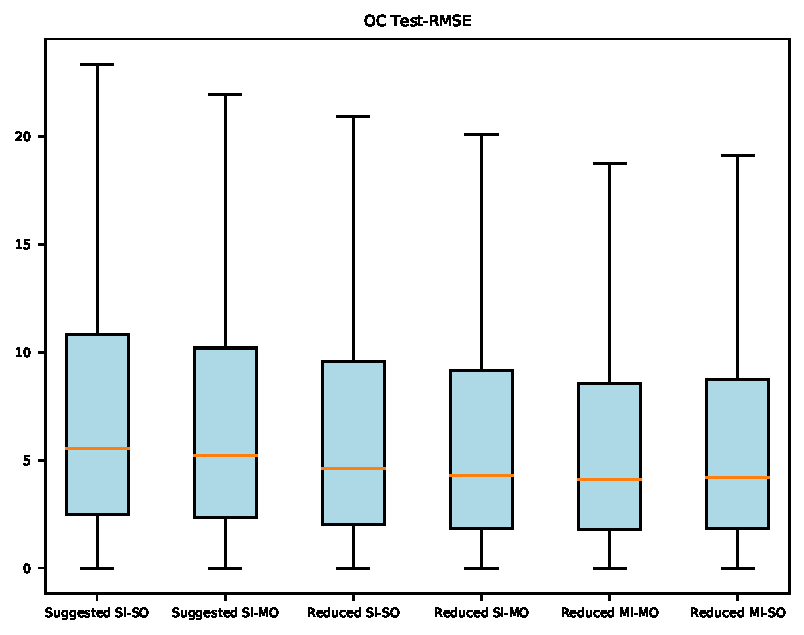
\includegraphics[width=1\linewidth]{RESULTS/BOXPLOTS/OC.pdf}
        \caption{Σύγκριση μοντέλων για την ιδιότητα του οργανικού άνθρακα}
        \label{fig:OC_boxplot}
    \end{subfigure}
    \begin{subfigure}{0.5\textwidth}
        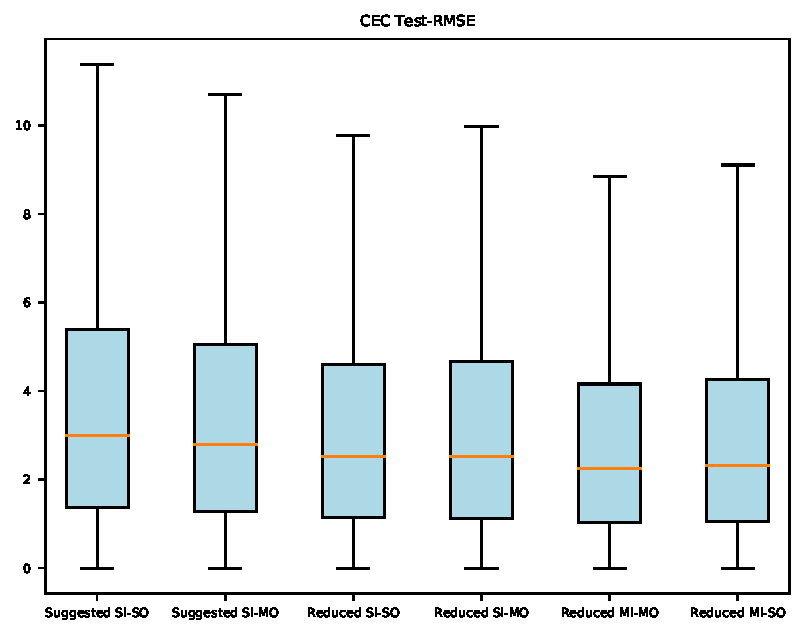
\includegraphics[width=1\linewidth]{RESULTS/BOXPLOTS/CEC.pdf}
        \caption{Σύγκριση μοντέλων για την ιδιότητα της ικανότητας ανταλλαγής κατιόντων}
        \label{fig:CEC_boxplot}
    \end{subfigure}
    \caption{Θηκογράμματα απόλυτου σφάλματος για τις ιδιότητες \tl{OC} και \tl{CEC}}
\end{figure}
\begin{figure}[H]
    \begin{subfigure}{0.5\textwidth}
        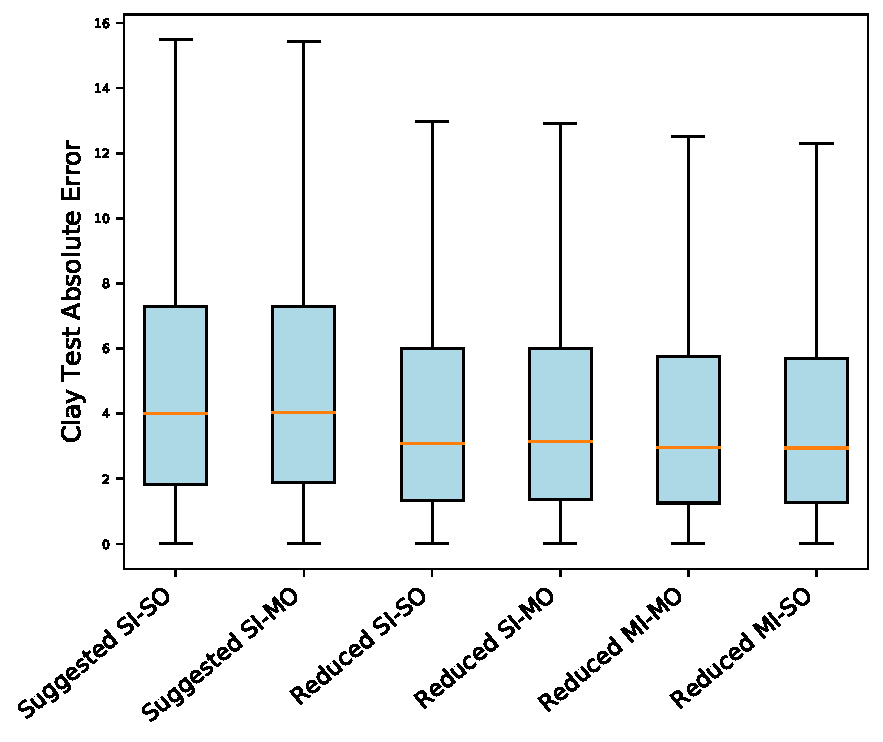
\includegraphics[width=1\linewidth]{RESULTS/BOXPLOTS/Clay.pdf}
        \caption{Σύγκριση μοντέλων για την ιδιότητα την περιεκτικότητα σε άργιλο}
        \label{fig:Clay_boxplot}
    \end{subfigure}
    \begin{subfigure}{0.5\textwidth}
        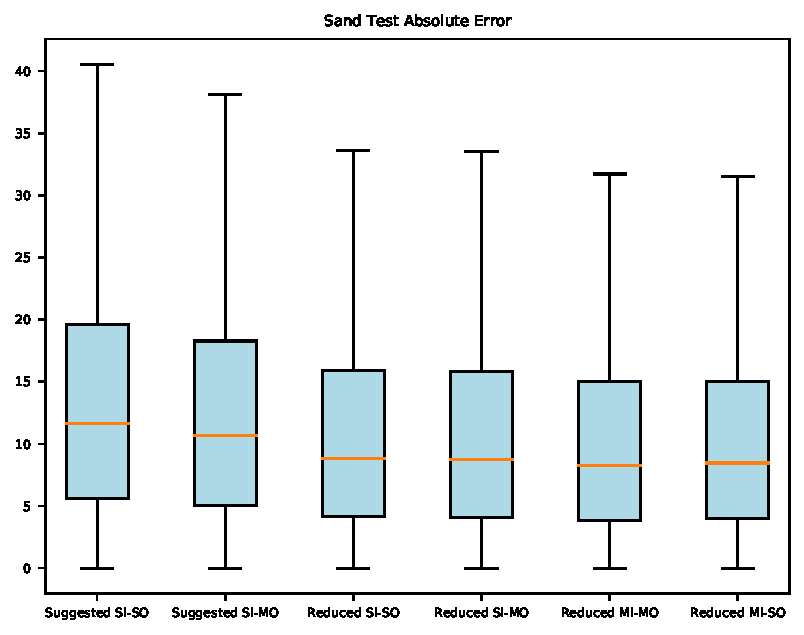
\includegraphics[width=1\linewidth]{RESULTS/BOXPLOTS/Sand.pdf}
        \caption{Σύγκριση μοντέλων για την ιδιότητα την περιεκτικότητα σε άμμο}
        \label{fig:Sand_boxplot}
    \end{subfigure}
    \caption{Θηκογράμματα απόλυτου σφάλματος για τις ιδιότητες \tl{Clay} και \tl{Sand}}
\end{figure}
\begin{figure}[H]
    \begin{subfigure}{0.5\textwidth}
        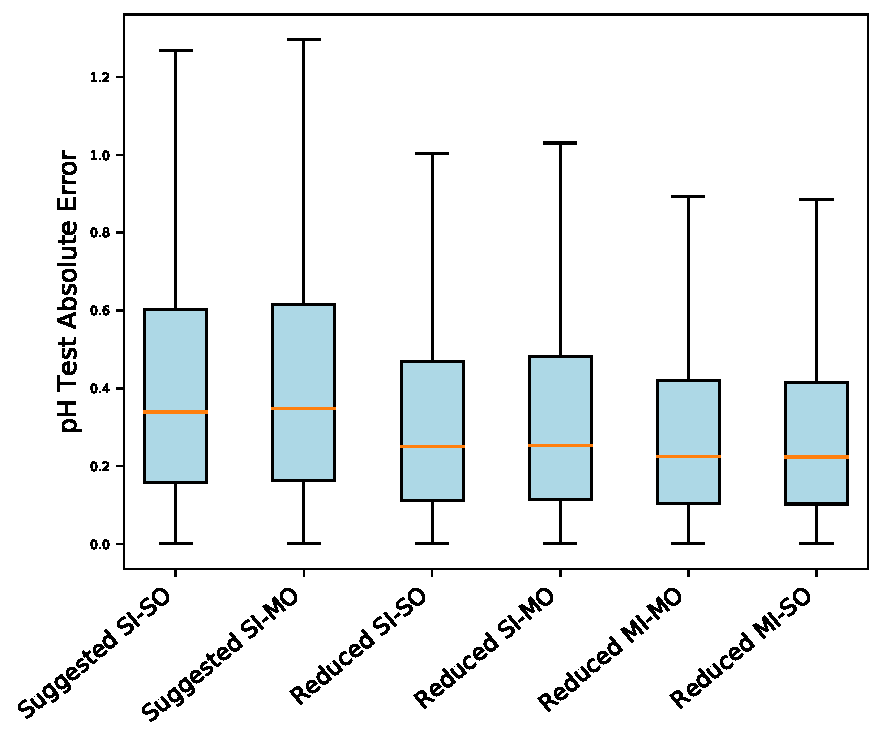
\includegraphics[width=1\linewidth]{RESULTS/BOXPLOTS/pH.pdf}
        \caption{Σύγκριση μοντέλων για την ιδιότητα την περιεκτικότητα του \tl{pH} στο νερό}
        \label{fig:pH_boxplot}
    \end{subfigure}
    \begin{subfigure}{0.5\textwidth}
        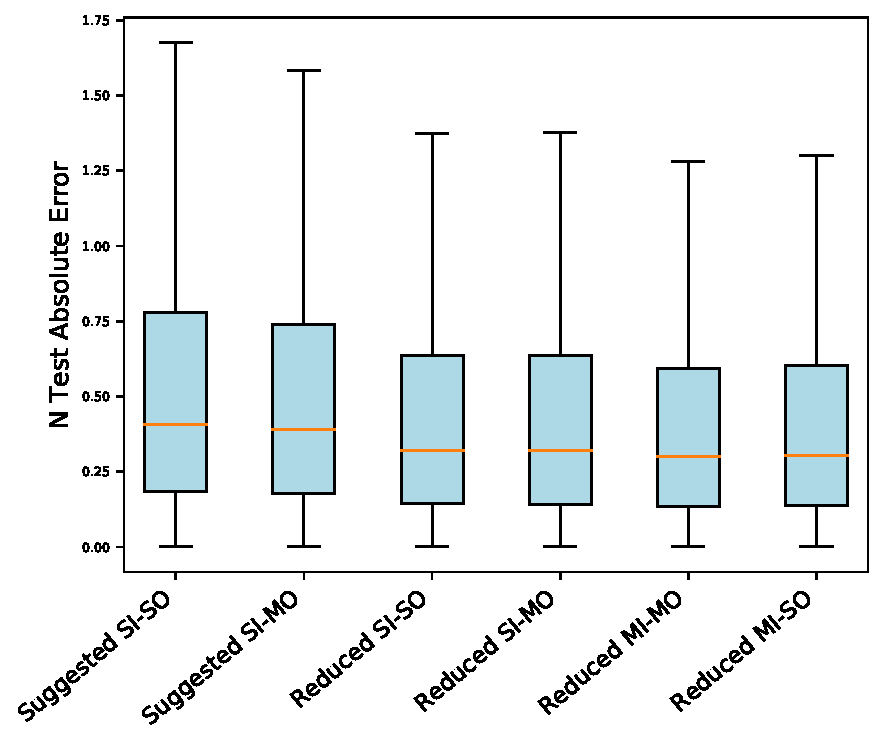
\includegraphics[width=1\linewidth]{RESULTS/BOXPLOTS/N.pdf}
        \caption{Σύγκριση μοντέλων για την ιδιότητα της περιεκτικότητας του αζώτου στο έδαφος}
        \label{fig:N_boxplot}
    \end{subfigure}
    \caption{Θηκογράμματα απόλυτου σφάλματος για τις ιδιότητες \tl{pH} και \tl{N}}
\end{figure}
\begin{figure}[H]
    \begin{subfigure}{0.5\textwidth}
        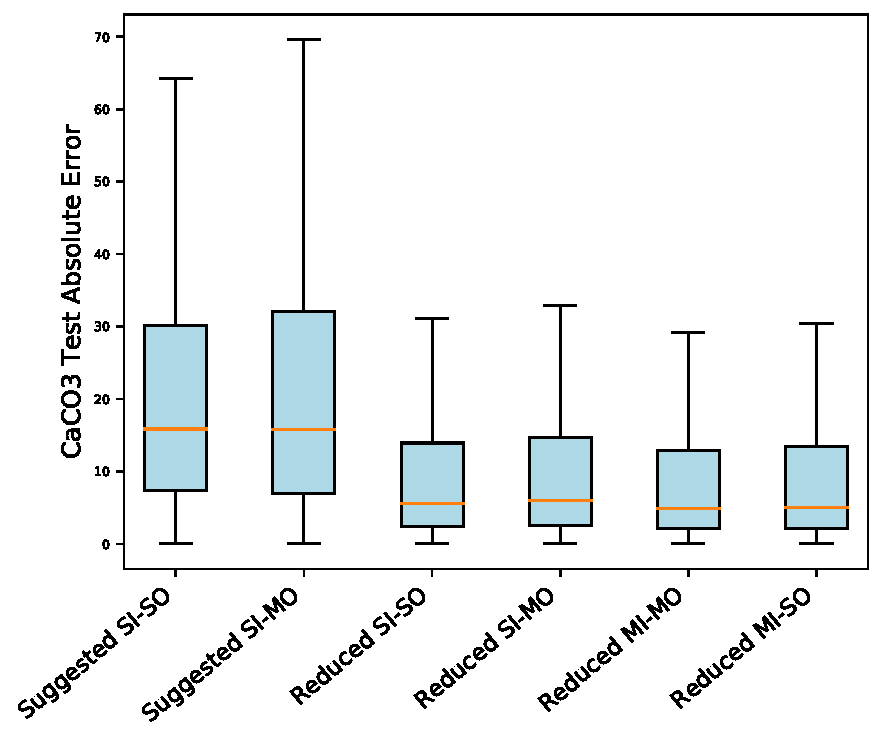
\includegraphics[width=1\linewidth]{RESULTS/BOXPLOTS/CaCO3.pdf}
        \caption{Σύγκριση μοντέλων για την ιδιότητα την περιεκτικότητα ανθρακικού ασβεστίου στο έδαφος}
        \label{fig:CaCO3_boxplot}
    \end{subfigure}
    \begin{subfigure}{0.5\textwidth}
        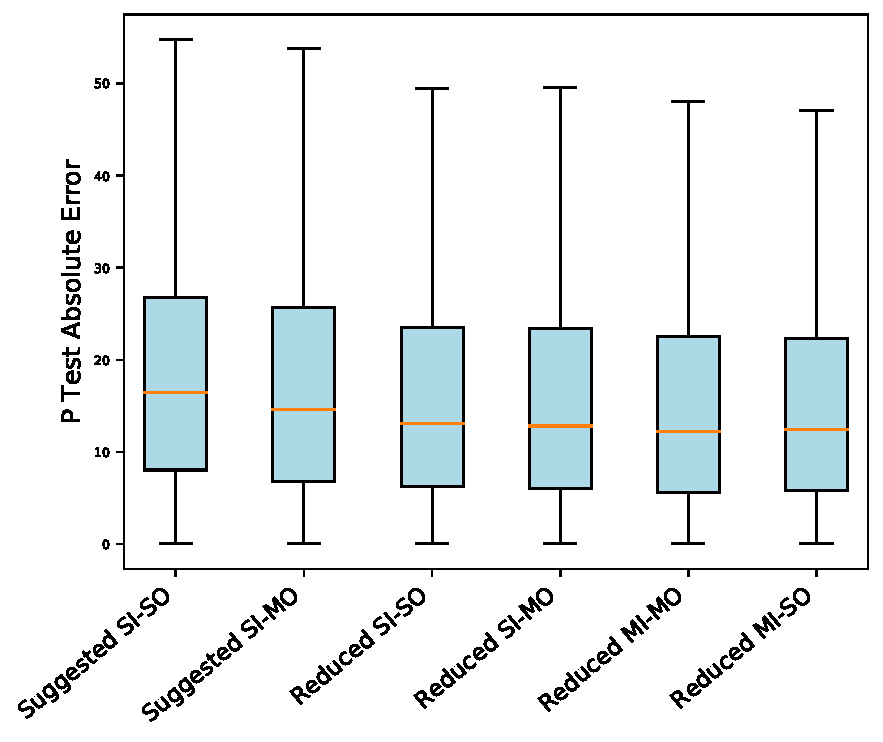
\includegraphics[width=1\linewidth]{RESULTS/BOXPLOTS/P.pdf}
        \caption{Σύγκριση μοντέλων για την ιδιότητα της περιεκτικότητας του φωσφόρου στο έδαφος}
        \label{fig:P_boxplot}
    \end{subfigure}
    \caption{Θηκογράμματα απόλυτου σφάλματος για τις ιδιότητες \tl{CaCO3} και \tl{P}}
\end{figure}
\begin{figure}[H]
    \begin{subfigure}{0.5\textwidth}
        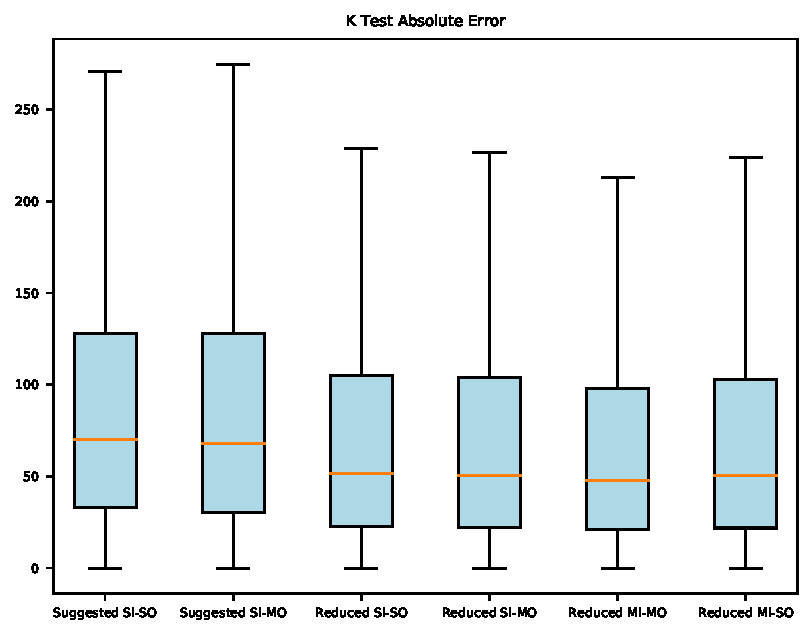
\includegraphics[width=1\linewidth]{RESULTS/BOXPLOTS/K.pdf}
        \caption{Σύγκριση μοντέλων για την ιδιότητα την περιεκτικότητα του καλίου στο έδαφος}
        \label{fig:K_boxplot}
    \end{subfigure}
    \begin{subfigure}{0.5\textwidth}
        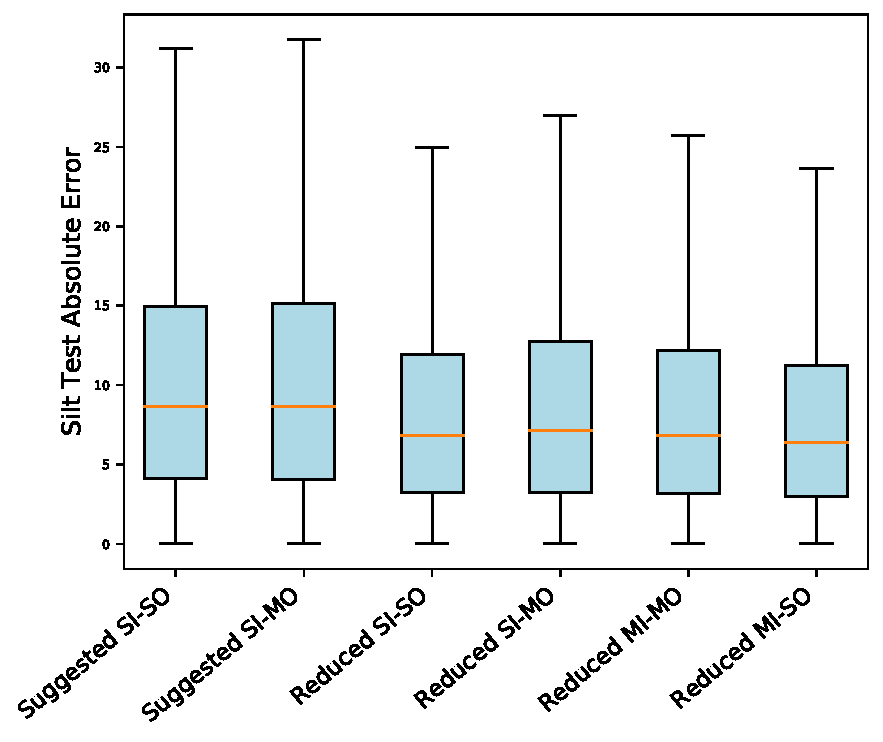
\includegraphics[width=1\linewidth]{RESULTS/BOXPLOTS/Silt.pdf}
        \caption{Σύγκριση μοντέλων για την ιδιότητα την περιεκτικότητα του εδάφους σε ιλύ}
        \label{fig:Silt_boxplot}
    \end{subfigure}
    \caption{Θηκογράμματα απόλυτου σφάλματος για τις ιδιότητες \tl{K} και \tl{Silt}}
\end{figure}

Στα παράπανω θηκογράμματα φαίνεται πως η επίδοση των βέλτιστων μοντέλων είναι αισθητά καλύτερη από αυτή των προτεινόμενων κάτι που εξακριβώνεται από την θέση της διαμέσου $Q_{50}$ αλλά και της μορφής του διαστήματος μεταξύ του 3ου $Q_{75}$ τεταρτημορίου και του μέγιστου σφάλματος. Ανάμεσα στα μοντέλα της βέλτιστης αρχιτεκτονικής φαίνεται πως η χρήση πολλαπλών εισόδων έχει αυξημένες επιδόσεις σε σχέση με αυτά της μονής εισόδου σπεκτρογράμματος ανακλαστικότητας για αρκετές από τις ιδιότητες.

\begin{figure}[H]
    \begin{subfigure}{0.5\textwidth}
        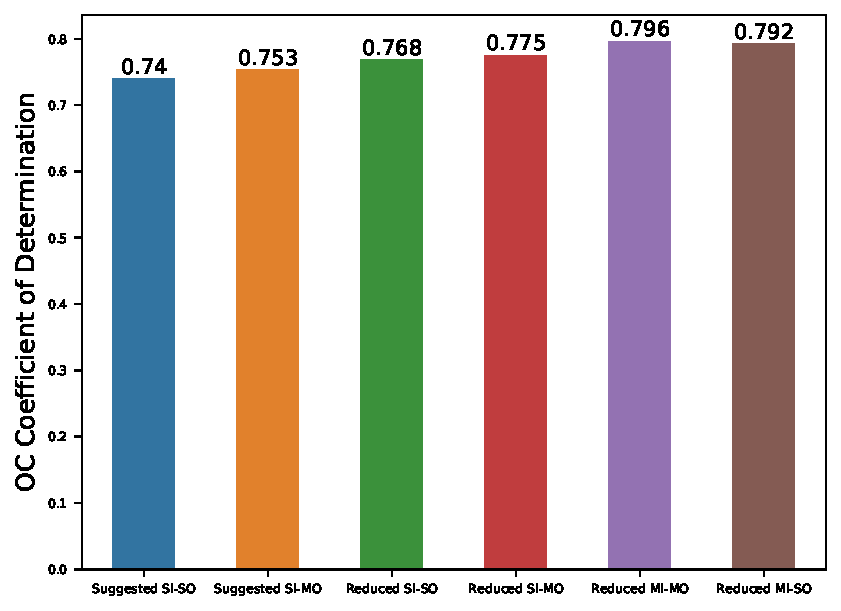
\includegraphics[width=1\linewidth]{RESULTS/BARPLOTS/test_OC_determ.pdf}
        \caption{Σύγκριση μοντέλων για την ιδιότητα του οργανικού άνθρακα}
        \label{fig:OC_determ}
    \end{subfigure}
    \begin{subfigure}{0.5\textwidth}
        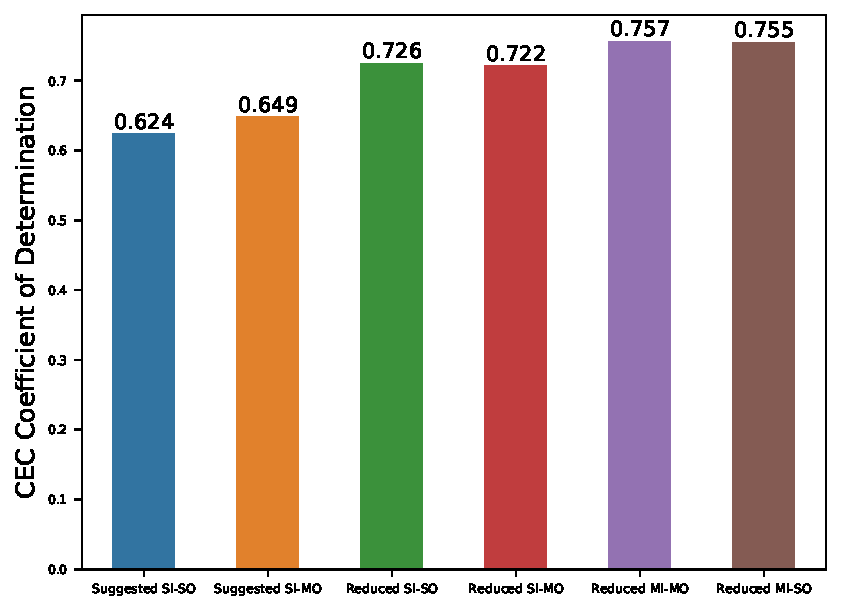
\includegraphics[width=1\linewidth]{RESULTS/BARPLOTS/test_CEC_determ.pdf}
        \caption{Σύγκριση μοντέλων για την ιδιότητα της ικανότητας ανταλλαγής κατιόντων}
        \label{fig:CEC_determ}
    \end{subfigure}
    \caption{Ραβδογράμματα συντελεστή προσδιορισμού για τις ιδιότητες \tl{OC} και \tl{CEC}}
\end{figure}
\begin{figure}[H]
    \begin{subfigure}{0.5\textwidth}
        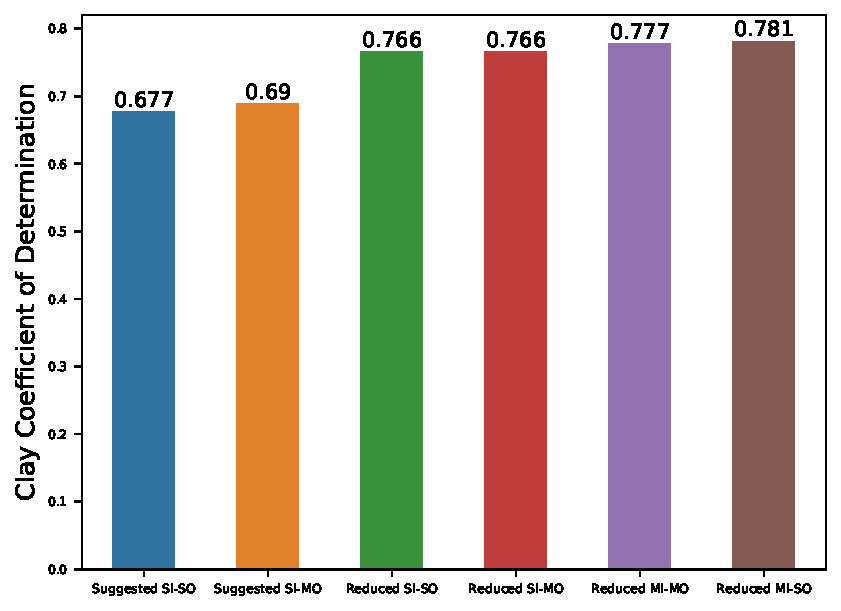
\includegraphics[width=1\linewidth]{RESULTS/BARPLOTS/test_Clay_determ.pdf}
        \caption{Σύγκριση μοντέλων για την ιδιότητα την περιεκτικότητα σε άργιλο}
        \label{fig:Clay_determ}
    \end{subfigure}
    \begin{subfigure}{0.5\textwidth}
        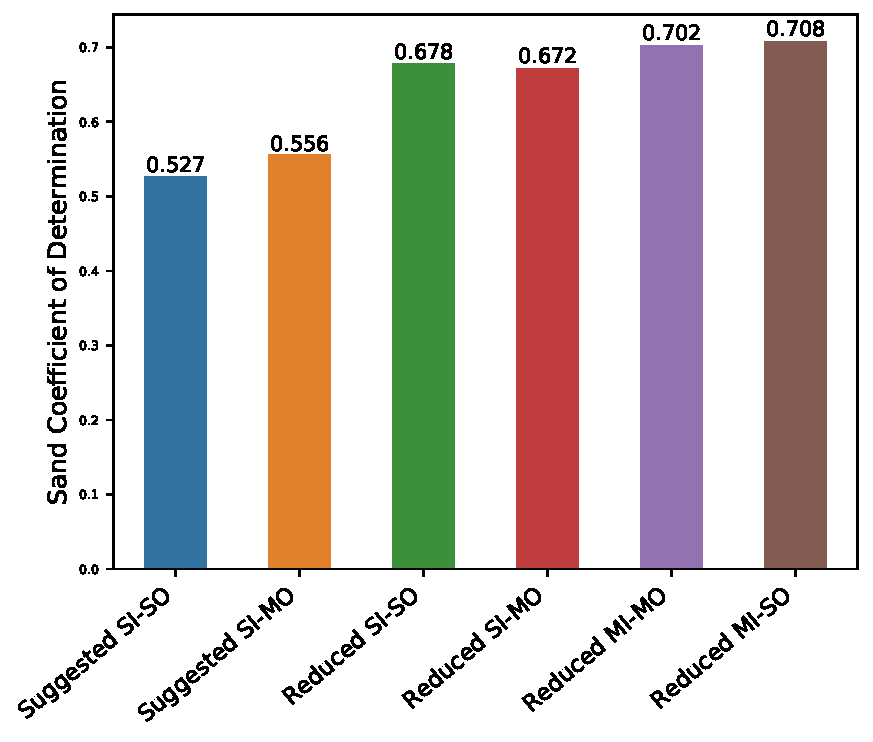
\includegraphics[width=1\linewidth]{RESULTS/BARPLOTS/test_Sand_determ.pdf}
        \caption{Σύγκριση μοντέλων για την ιδιότητα την περιεκτικότητα σε άμμο}
        \label{fig:Sand_determ}
    \end{subfigure}
    \caption{Ραβδογράμματα συντελεστή προσδιορισμού για τις ιδιότητες \tl{Clay} και \tl{Sand}}
\end{figure}
\begin{figure}[H]
    \begin{subfigure}{0.5\textwidth}
        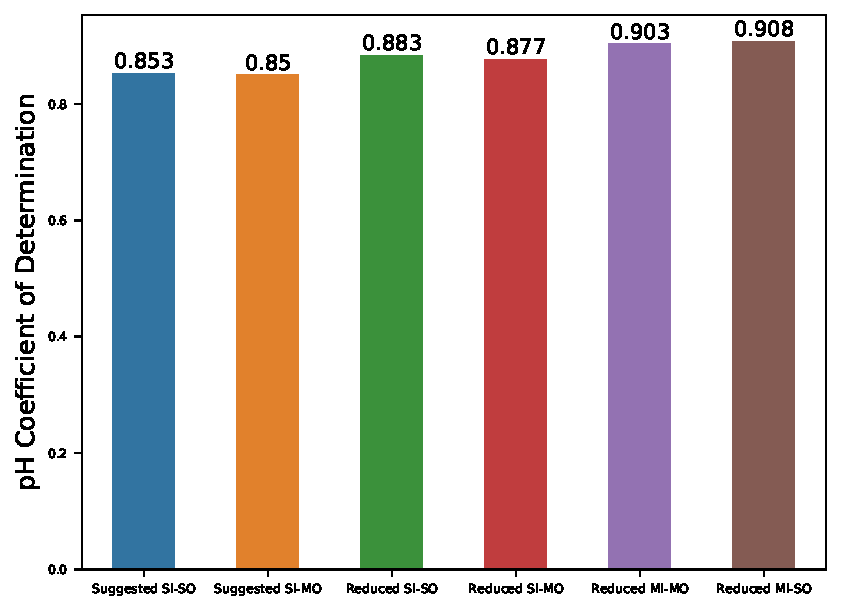
\includegraphics[width=1\linewidth]{RESULTS/BARPLOTS/test_pH_determ.pdf}
        \caption{Σύγκριση μοντέλων για την ιδιότητα την περιεκτικότητα του \tl{pH} στο νερό}
        \label{fig:pH_determ}
    \end{subfigure}
    \begin{subfigure}{0.5\textwidth}
        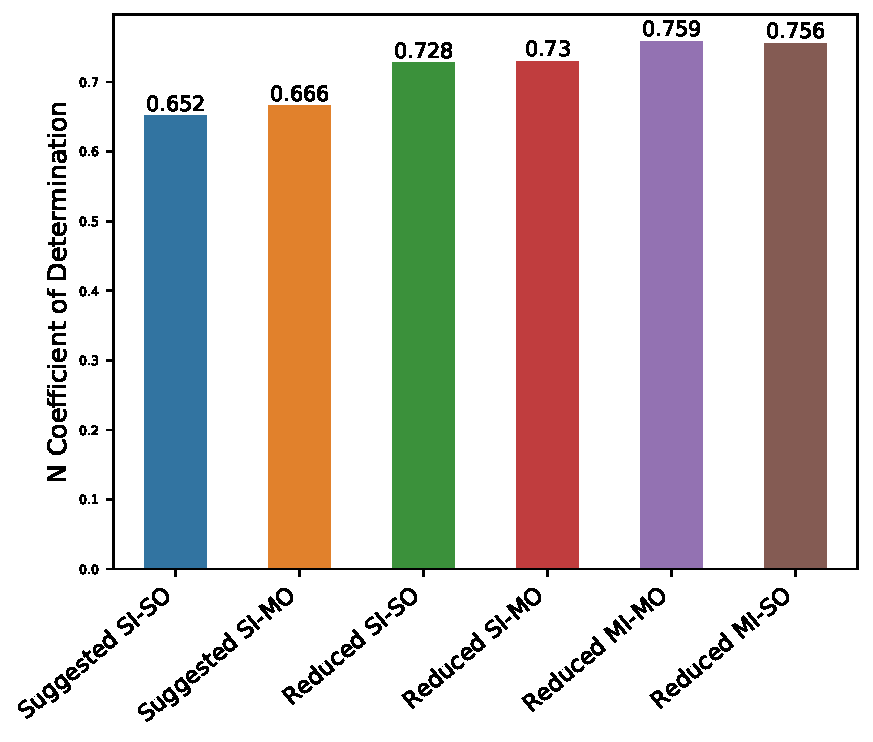
\includegraphics[width=1\linewidth]{RESULTS/BARPLOTS/test_N_determ.pdf}
        \caption{Σύγκριση μοντέλων για την ιδιότητα της περιεκτικότητας του αζώτου στο έδαφος}
        \label{fig:N_determ}
    \end{subfigure}
    \caption{Ραβδογράμματα συντελεστή προσδιορισμού για τις ιδιότητες \tl{pH} και \tl{N}}
\end{figure}
\begin{figure}[H]
    \begin{subfigure}{0.5\textwidth}
        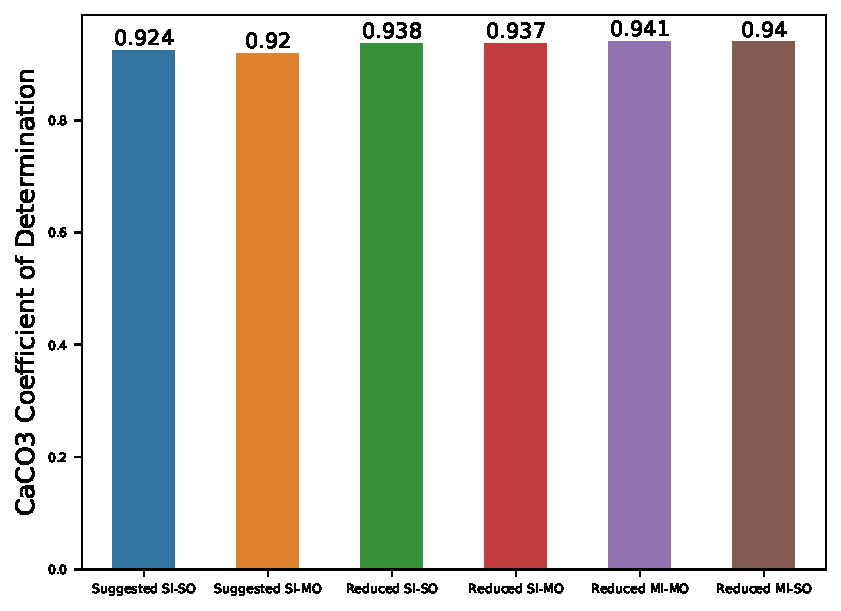
\includegraphics[width=1\linewidth]{RESULTS/BARPLOTS/test_CaCO3_determ.pdf}
        \caption{Σύγκριση μοντέλων για την ιδιότητα την περιεκτικότητα ανθρακικού ασβεστίου στο έδαφος}
        \label{fig:CaCO3_determ}
    \end{subfigure}
    \begin{subfigure}{0.5\textwidth}
        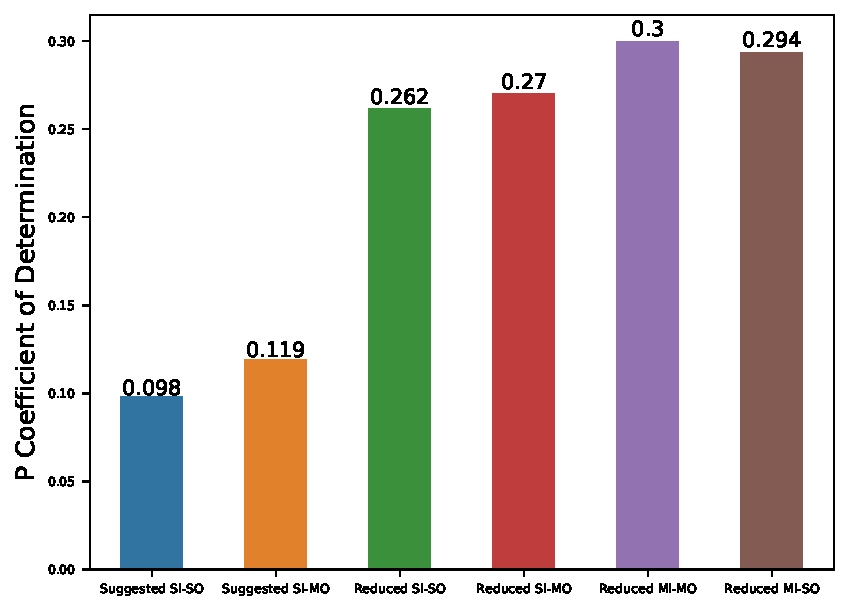
\includegraphics[width=1\linewidth]{RESULTS/BARPLOTS/test_P_determ.pdf}
        \caption{Σύγκριση μοντέλων για την ιδιότητα της περιεκτικότητας του φωσφόρου στο έδαφος}
        \label{fig:P_determ}
    \end{subfigure}
    \caption{Ραβδογράμματα συντελεστή προσδιορισμού για τις ιδιότητες \tl{CaCO3} και \tl{P}}
\end{figure}
\begin{figure}[H]
    \begin{subfigure}{0.5\textwidth}
        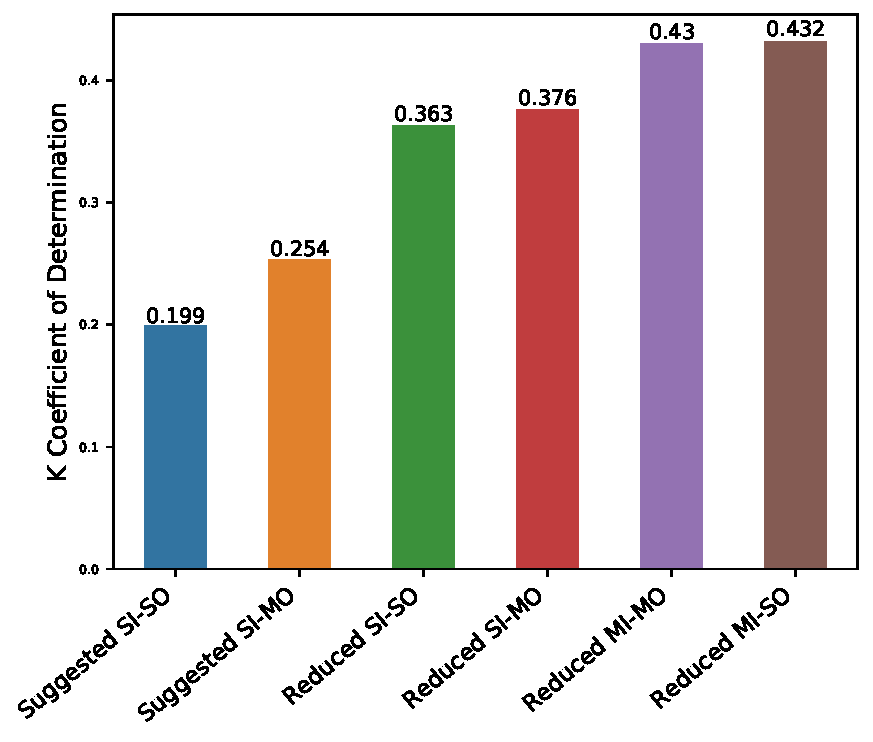
\includegraphics[width=1\linewidth]{RESULTS/BARPLOTS/test_K_determ.pdf}
        \caption{Σύγκριση μοντέλων για την ιδιότητα την περιεκτικότητα του καλίου στο έδαφος}
        \label{fig:K_determ}
    \end{subfigure}
    \begin{subfigure}{0.5\textwidth}
        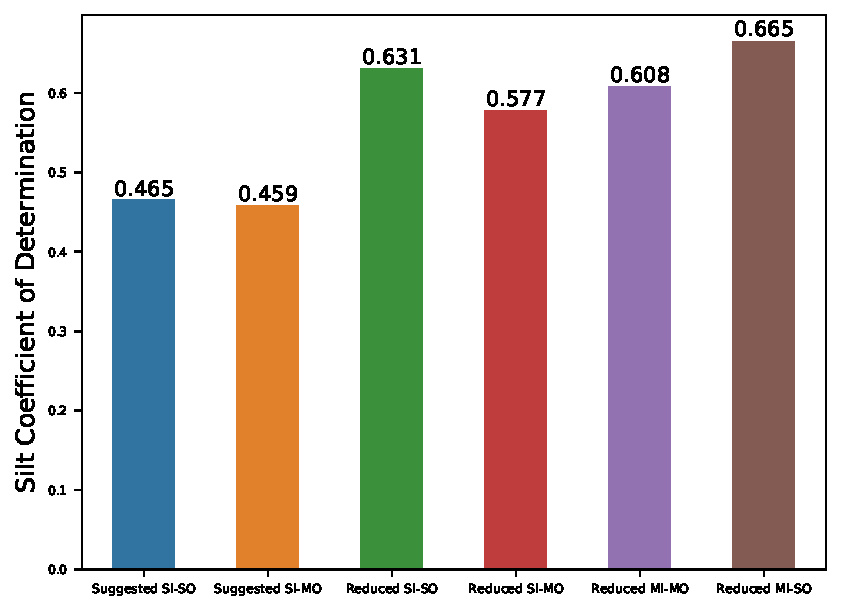
\includegraphics[width=1\linewidth]{RESULTS/BARPLOTS/test_Silt_determ.pdf}
        \caption{Σύγκριση μοντέλων για την ιδιότητα την περιεκτικότητα του εδάφους σε ιλύ}
        \label{fig:Silt_determ}
    \end{subfigure}
    \caption{Ραβδογράμματα συντελεστή προσδιορισμού για τις ιδιότητες \tl{K} και \tl{Silt}}
\end{figure}

\todo{Σχολιασμός}

\section{Οπτικοποίηση συνελικτικών φίλτρων του μοντέλου}
Η φύση των δισδιάστατων νευρωνικών δικτύων τα καθιστά κατάλληλα για πειραματισμούς σχετικά με την μορφή της εισόδου που εισέρχεται στο μοντέλο σε κάθε επίπεδο του. Σε κάποιες περιπτώσεις οι μορφές των συνελικτικών φίλτρων θα μπορούσαν να ερμηνευτούν αναλόγως με τα χαρακτηριστικά που αφορούν την μορφή της εισόδου και την πληροφορία που αποσκοπείται να εξαχθεί από αυτή. Στην περίπτωση της εισόδου των μοντέλων που πραγματεύεται η παρούσα διπλωματική εργασία, τα μοτίβα που ανιχνεύονται στα σπεκτρογράμματα είναι ίσως κάποιες συγκεκριμένες διακυμάνσεις στις φασματικές υπογραφές και στους μετασχηματισμούς \tl{wavelet}.

Για την οπτικοποίηση των ενεργοποιήσεων των διαφόρων επιπέδων του μοντέλου εκπαιδεύεται ένα μοντέλο μιας εισόδου και μιας εξόδου, συγκεκριμένα  με τη χρήση φασματικών υπογραφών ανακλαστικότητας και με έξοδο την περιεκτικότητα σε οργανικό άνθρακα. Στη συνέχεια παρατίθενται οι μορφές των εξόδων κάθε επιπέδου από την είσοδο μέχρι το σημείο του μοντέλου όπου τα δεδομένα είναι σε δισδιάστατη μορφή.
\textit{Διαγραμμάτα}
\begin{figure}[H]
  \begin{center}
    \includesvg[width=1\textwidth]{RESULTS/model_layer_0_OC_input_3}
    \caption{Είσοδος μετά την μετατροπή σε σπεκτρόγραμμα από φασματική υπογραφή ανακλαστικότητας}
  \end{center}
\end{figure}

%\begin{figure}[htbp]
%    \begin{subfigure}{0.5\textwidth}
        %\includesvg[width=1\linewidth]{RESULTS/model_layer_1_OC_conv2d_4}
        %\caption{Πραγματικές τιμές}
        %\label{fig:subim1}
%    \end{subfigure}
%    \begin{subfigure}{0.5\textwidth}
        %\includesvg[width=1\linewidth]{RESULTS/model_layer_1_OC_conv2d_4_standarized}
        %\caption{Κανονικοποιημένες τιμές}
        %\label{fig:subim1}
%    \end{subfigure}
%    \caption{Μορφή της εξόδου του πρώτου δισδιάστατου συνελικτικού επιπέδου. Έξοδος για τα πρώτα 18 \tl{Feature %Maps}}
%\end{figure}
%
%\begin{figure}[H]
%  \begin{center}
%    \includesvg[width=0.3\textwidth]{RESULTS/model_layer_1_OC_conv2d_4_kernels}
%    \caption{Μορφή των συνελικιτκών φίλτρων που χρησιμοποιήθηκαν από το πρώτο δισδιάστατο συνελικτικό επιπέδο. %Φαίνονται τα  18 πρώτα φίλτρα}
%  \end{center}
%\end{figure}

\begin{figure}[H]
    \begin{subfigure}{0.7\textwidth}
        \begin{subfigure}{\textwidth}
            \includesvg[width=1\linewidth]{RESULTS/model_layer_1_OC_conv2d_4}
            \caption{Πραγματικές τιμές}
            \label{fig:layer_1}
        \end{subfigure}
        \begin{subfigure}{\textwidth}
            \includesvg[width=1\linewidth]{RESULTS/model_layer_1_OC_conv2d_4_standarized}
            \caption{Κανονικοποιημένες τιμές}
            \label{fig:layer_1_stand}
        \end{subfigure}
    \end{subfigure}
    \begin{subfigure}{0.3\textwidth}
        \includesvg[width=\textwidth]{RESULTS/model_layer_1_OC_conv2d_4_kernels}
        \caption{Μορφή των συνελικιτκών φίλτρων που χρησιμοποιήθηκαν από το πρώτο δισδιάστατο συνελικτικό επιπέδο. Φαίνονται τα  18 πρώτα φίλτρα}
        \label{fig:layer_1_filters}
    \end{subfigure}
    \caption{Μορφή της εξόδου του πρώτου δισδιάστατου συνελικτικού επιπέδου. Έξοδος για τα πρώτα 18 \tl{Feature Maps}}
\end{figure}

\begin{figure}[H]
    \begin{subfigure}{0.5\textwidth}
        \includesvg[width=1\linewidth]{RESULTS/model_layer_2_OC_batch_normalization_8}
        \caption{Πραγματικές τιμές}
        \label{fig:layer_2}
    \end{subfigure}
    \begin{subfigure}{0.5\textwidth}
        \includesvg[width=1\linewidth]{RESULTS/model_layer_2_OC_batch_normalization_8_standarized}
        \caption{Κανονικοποιημένες τιμές}
        \label{fig:layer_2_stand}
    \end{subfigure}
    \caption{Μορφή της εξόδου μετά το επίπεδο της κανονικοποίησης παρτίδας. Έξοδος για τα πρώτα 18 \tl{Feature Maps}}
\end{figure}

\begin{figure}[H]
    \begin{subfigure}{0.5\textwidth}
        \includesvg[width=1\linewidth]{RESULTS/model_layer_3_OC_re_lu_8}
        \caption{Πραγματικές τιμές}
        \label{fig:layer_3}
    \end{subfigure}
    \begin{subfigure}{0.5\textwidth}
        \includesvg[width=1\linewidth]{RESULTS/model_layer_3_OC_re_lu_8_standarized}
        \caption{Κανονικοποιημένες τιμές}
        \label{fig:layer_3_stand}
    \end{subfigure}
    \caption{Μορφή της εξόδου του πρώτου δισδιάστατου συνελικτικού επιπέδου μετά την συνάρτηση ενεργοποίησης \tl{ReLU}. Έξοδος για τα πρώτα 18 \tl{Feature Maps}}
\end{figure}

\begin{figure}[H]
    \begin{subfigure}{0.5\textwidth}
        \includesvg[width=1\linewidth]{RESULTS/model_layer_4_OC_max_pooling2d_2}
        \caption{Πραγματικές τιμές}
        \label{fig:layer_4}
    \end{subfigure}
    \begin{subfigure}{0.5\textwidth}
        \includesvg[width=1\linewidth]{RESULTS/model_layer_4_OC_max_pooling2d_2_standarized}
        \caption{Κανονικοποιημένες τιμές}
        \label{fig:layer_4_stand}
    \end{subfigure}
    \caption{Μορφή της εξόδου μετά την συνάρτηση ενεργοποίησης \tl{ReLU} του πρώτου επιπέδου και της εφαρμογής συγκέντρωσης μεγίστων. Έξοδος για τα πρώτα 18 \tl{Feature Maps}}
\end{figure}


\begin{figure}[H]
    \begin{subfigure}{0.7\textwidth}
        \begin{subfigure}{\textwidth}
            \includesvg[width=1\linewidth]{RESULTS/model_layer_5_OC_conv2d_5}
            \caption{Πραγματικές τιμές}
            \label{fig:layer_5}
        \end{subfigure}
        \begin{subfigure}{\textwidth}
            \includesvg[width=1\linewidth]{RESULTS/model_layer_5_OC_conv2d_5_standarized}
            \caption{Κανονικοποιημένες τιμές}
            \label{fig:layer_5_stand}
        \end{subfigure}
    \end{subfigure}
    \begin{subfigure}{0.3\textwidth}
        \includesvg[width=\textwidth]{RESULTS/model_layer_5_OC_conv2d_5_kernels}
        \caption{Μορφή των συνελικιτκών φίλτρων που χρησιμοποιήθηκαν από το δεύτερο δισδιάστατο συνελικτικό επιπέδο. Φαίνονται τα  18 πρώτα φίλτρα}
        \label{fig:layer_5_filters}
    \end{subfigure}
    \caption{Μορφή της εξόδου του δευτερου δισδιάστατου συνελικτικού επιπέδου. Έξοδος για τα πρώτα 18 \tl{Feature Maps}}
\end{figure}

%\begin{figure}[htbp]
    %\begin{subfigure}{0.5\textwidth}
        %\includesvg[width=1\linewidth]{RESULTS/model_layer_5_OC_conv2d_5}
        %\caption{Πραγματικές τιμές}
        %\label{fig:subim7}
    %\end{subfigure}
    %\begin{subfigure}{0.5\textwidth}
        %\includesvg[width=1\linewidth]{RESULTS/model_layer_5_OC_conv2d_5_standarized}
        %\caption{Κανονικοποιημένες τιμές}
        %\label{fig:subim8}
    %\end{subfigure}
    %\caption{Μορφή της εξόδου του δευτερου δισδιάστατου συνελικτικού επιπέδου. Έξοδος για τα πρώτα 18 %\tl{Feature Maps}}
%\end{figure}
%
%\begin{figure}[H]
  %\begin{center}
%    \includesvg[width=0.3\textwidth]{RESULTS/model_layer_5_OC_conv2d_5_kernels}
%    \caption{Μορφή των συνελικιτκών φίλτρων που χρησιμοποιήθηκαν από το δεύτερο δισδιάστατο συνελικτικό επιπέδο. Φαίνονται τα  18 πρώτα φίλτρα}
  %\end{center}
%\end{figure}

\begin{figure}[H]
    \begin{subfigure}{0.5\textwidth}
        \includesvg[width=1\linewidth]{RESULTS/model_layer_6_OC_batch_normalization_9}
        \caption{Πραγματικές τιμές}
        \label{fig:layer_6}
    \end{subfigure}
    \begin{subfigure}{0.5\textwidth}
        \includesvg[width=1\linewidth]{RESULTS/model_layer_6_OC_batch_normalization_9_standarized}
        \caption{Κανονικοποιημένες τιμές}
        \label{fig:layer_6_stand}
    \end{subfigure}
    \caption{Μορφή της εξόδου μετά το επίπεδο της κανονικοποίησης παρτίδας του δεύτερου συνελικτικού επιπέδου. Έξοδος για τα πρώτα 18 \tl{Feature Maps}}
\end{figure}

\begin{figure}[H]
    \begin{subfigure}{0.5\textwidth}
        \includesvg[width=1\linewidth]{RESULTS/model_layer_7_OC_re_lu_9}
        \caption{Πραγματικές τιμές}
        \label{fig:layer_7}
    \end{subfigure}
    \begin{subfigure}{0.5\textwidth}
        \includesvg[width=1\linewidth]{RESULTS/model_layer_7_OC_re_lu_9_standarized}
        \caption{Κανονικοποιημένες τιμές}
        \label{fig:layer_7_stand}
    \end{subfigure}
    \caption{Μορφή της εξόδου του δεύτερου δισδιάστατου συνελικτικού επιπέδου μετά την συνάρτηση ενεργοποίησης \tl{ReLU}. Έξοδος για τα πρώτα 18 \tl{Feature Maps}}
\end{figure}

Στις παραπάνω εικόνες φαίνεται ο τρόπος με τον οποίο ένα μοντέλο το οποίο έχει προηγουμένως εκπαιδευτεί, επεξεργάζεται την μονοκαναλική εικόνα εισόδου σε όλα τα επίπεδα τα οποία έχει δισδιάστατη μορφή.\\

Στα δισδιάστατα συνελικτικά επίπεδα παρατηρείται πως η εικόνα εισόδου τροποποιείται σε διαφορετικές εκδοχές της ανάλογα με το συνελικτικό φίλτρο που εφαρμόζεται.\\

Στα επίπεδα κανονικιοποίησης παρτίδας είναι ορατή η κανονικοποίηση που υφίσταται το σύνολο των \tl{Feature Maps} σε σχέση με το εύρος τιμών που είχαν στα συνελικτικά επίπεδα.\\

Στα επίπεδα ενεργοποίησης με χρήση ανορθωμένης γραμμικής συνάρτησης \tl{ReLU} φαίνεται πως η εφαρμογή της συνάρτησης ενεργοποίσης επιτρέπει μόνο στα μέρη των εικόνων με μεγαλύτερες τιμές, τα οποία πιθανώς περιέχουν χρήσιμη πληροφορία, να μεταφερθούν προς το επόμενο επίπεδο.\\

Τα επίπεδα συγκέντρωσης μεγίστων τροποποιούν την είσοδο τους μειώνοντας τις διαστάσεις της ενώ διατηρούν τα μέγιστα των περιοχών τις οποίες συγκεντρώνουν. Το αποτέλεσμα οπτικά φαίνεται σαν μια σμίκρυνση της εικόνας εισόδου.\\

Κατά την επεξεργασία της εισόδου από το δισδιάστατο συνελικτικό νευρωνικό δίκτυο η μορφή της εικόνας τροποποιείται σημαντικά με αποτέλεσμα μετά το συνελικτικό επίπεδο 5 η εικόνα να μην έχει καμία ομοιότητα με την αρχική της μορφή.